% =============================================================================
% KALINGACONF 2026 — IEEE conference format (two-column)
% Track 1: Artificial Intelligence, Machine Learning, Blockchain, and
%          Cybersecurity  ->  "Ethical AI and Responsible Use" (FinTech)
%
% Length target: 6-8 body pages (conference max is 8, exclusive of bibliography),
% references push the total toward the proceedings' 10-page allocation.
%
% Every quantitative figure is a measured walk-forward statistic taken from the
% authors' deployed system; nothing is illustrative or simulated unless a caption
% explicitly says "conceptual".
% =============================================================================
\documentclass[conference]{IEEEtran}
\IEEEoverridecommandlockouts

\usepackage{cite}
\usepackage{amsmath,amssymb,amsfonts}
\usepackage{algorithm}
\usepackage{algorithmic}
\usepackage{graphicx}
\usepackage{textcomp}
\usepackage{xcolor}
\usepackage{booktabs}
\usepackage{array}
\usepackage{url}
\usepackage{tikz}
\usetikzlibrary{arrows.meta,positioning,calc,shapes.geometric}
\usepackage{pgfplots}
\pgfplotsset{compat=1.17}

\def\BibTeX{{\rm B\kern-.05em{\sc i\kern-.025em b}\kern-.08em
    T\kern-.1667em\lower.7ex\hbox{E}\kern-.125emX}}

\begin{document}

\title{Coverage Is the Price of Trust:\\
A Self-Auditing Honesty Contract for\\
Responsible AI in Equity Markets}

\author{
\IEEEauthorblockN{Anandkumar Pardeshi}
\IEEEauthorblockA{\textit{Dept.\ of Computer Science and Engineering} \\
\textit{Fr.\ C.\ Rodrigues Institute of Technology}\\
Vashi, Navi Mumbai, India \\
anand.pardeshi@fcrit.ac.in}
\and
\IEEEauthorblockN{Sujata Deshmukh}
\IEEEauthorblockA{\textit{Dept.\ of Computer Engineering} \\
\textit{Fr.\ C.\ Rodrigues Institute of Technology}\\
Vashi, Navi Mumbai, India \\
sujata.deshmukh@fcrit.ac.in}
}

\maketitle

% ---------------------------------------------------------------------------
\begin{abstract}
A financial AI that tells a retail user what to buy is a high-stakes,
outward-facing system, yet the literature evaluates such systems almost entirely
on accuracy and area under the curve (AUC). Those metrics say nothing about whether
a model knows when it is wrong. We argue that for a forecaster operating near the
efficient-market limit the right design objective is not accuracy but \emph{trust},
and that the currency in which trust is bought is \emph{coverage}: the fraction of
the time the system is willing to act. We make this concrete with the
\textbf{honesty contract}, a set of five machine-checkable, inference-time
invariants---calibrated confidence, conviction-gated abstention, a cost-aware alpha
gate, a Sharpe-triggered circuit breaker, and an append-only audit ledger---that
together turn a near-worthless ranker into a deployable adviser. On eight years of
National Stock Exchange of India (NSE) data we support each invariant with measured
numbers only. Next-period single-name direction is unpredictable beyond drift
(50.1\% out-of-sample, ranking AUC~$\approx$~0.47, confirmed five ways). A
three-stage calibration cuts expected calibration error (ECE) from 0.35 to 0.05
without moving accuracy. And a conviction gate that abstains on 94\% of
observations lifts the realized 30-trading-day hit-rate to 60.6\% against a 58.1\%
base rate, beating it in four of five test years. The contribution is a reusable,
auditable architecture for responsible financial AI, with evidence that under a
near-random discriminator value is recovered by abstaining rather than ranking, and
that the metric worth reporting is precision-at-coverage, not AUC.
\end{abstract}

\begin{IEEEkeywords}
responsible AI, selective prediction, abstention, probability calibration,
trustworthy machine learning, FinTech, conformal prediction, model monitoring
\end{IEEEkeywords}

% ===========================================================================
\section{Introduction}
% ===========================================================================
The machine-learning-for-finance literature has a credibility problem that is
easy to miss because it hides inside good news. Directional accuracies of
60--70\% are reported routinely, but they rarely survive three elementary checks:
are the predicted probabilities \emph{calibrated}, does the evaluation
\emph{respect the arrow of time}, and are realistic transaction costs charged on
every round trip? A long methodological literature has shown how easily these
omissions manufacture phantom skill, whether through backtest overfitting
\cite{bailey2014}, multiple-testing selection \cite{harvey2016}, or simply the
absence of a disciplined protocol \cite{arnott2019,lopezdeprado2018}. When we ran
the same checks against our own deployed platform, the comfortable numbers
evaporated. This paper is an account of what we built once they did.

The deeper issue is one of framing. A system that tells a retail investor to buy a
stock is not a benchmark entry; it is an outward-facing decision aid whose mistakes
cost real money and whose confidence is read literally by non-experts. In an
emerging market such as India, driven by foreign and domestic institutional flows
and a large, news-sensitive retail base, the asymmetry is stark: the user bears the
downside of every overconfident call. Accuracy is the wrong headline metric here,
because a model can be accurate on average and still be dangerously overconfident on
exactly the cases a user acts on. What matters is whether the system knows the
limits of its own knowledge, and whether it is willing to say nothing when it knows
nothing. Responsible-AI scholarship has named these properties (transparency,
accountability, the duty to abstain \cite{jobin2019,amodei2016,mitchell2019}), but
mostly as principles. The practitioner is left without a concrete, checkable
specification of what a trustworthy financial predictor must actually \emph{do} at
inference time.

We close that gap with the \textbf{honesty contract}: a small set of invariants
that a deployed forecaster must satisfy on \emph{every} prediction, each enforced
by a specific software control and each costing the system some of its willingness
to act. The contract reframes trustworthy forecasting as a
\emph{selective-prediction} problem \cite{chow1970,elyaniv2010,geifman2017}: the
model is allowed, even encouraged, to abstain, and is judged not by how it ranks
every opportunity but by how reliable it is on the few it chooses to act on. This
framing fits emerging-market equities well, since the efficient-market hypothesis
\cite{fama1970} already predicts that short-horizon single-name direction should be
close to unpredictable, and our own measurements bear that out.

\noindent\textbf{Contributions.}
\begin{enumerate}
\item We formalize the \emph{honesty contract}: five machine-checkable,
inference-time invariants---calibrated confidence, conviction-gated abstention, a
cost-aware alpha gate, a Sharpe-triggered circuit breaker, and an append-only
audit ledger---that constitute a reusable architecture for responsible financial
AI (Section~\ref{sec:contract}).
\item We give a selective-prediction formalization in which each invariant
\emph{spends coverage to buy trust}, and argue that when discriminative power is
near random the correct evaluation lens is \emph{precision-at-coverage}, not
accuracy or AUC (Sections~\ref{sec:contract} and \ref{sec:tradeoff}).
\item We provide a fully reproducible eight-year NSE case study in which every
reported quantity is a measured walk-forward statistic, including a verified
accuracy ceiling confirmed five ways and a live circuit breaker tied to realized
Sharpe (Sections~\ref{sec:system}--\ref{sec:results}).
\item We show that a ranker with AUC~$\approx$~0.47---below chance---still yields a
usable, year-on-year-stable $+2.6$-point precision edge once value is harvested
from its extreme-conviction tail by abstention rather than ranking
(Section~\ref{sec:tradeoff}).
\end{enumerate}

% ===========================================================================
\section{Related Work}
% ===========================================================================
\textbf{Calibration of probabilistic forecasts.} A probability is trustworthy only
if it matches observed frequency. Modern high-capacity models are systematically
miscalibrated \cite{guo2017}; the classical remedies---Platt scaling
\cite{platt1999}, isotonic regression \cite{zadrozny2002}, and the empirical
analysis of when each helps \cite{niculescu2005}---are well understood, and the
Brier score \cite{brier1950} together with expected calibration error (ECE)
quantify the gap. The point under-appreciated in applied finance is that
calibration and discrimination are \emph{orthogonal}: a model with no edge can
still be made honest, and an accurate model can still lie about its confidence. Our
first invariant operationalizes exactly this separation.

\textbf{Selective prediction and the reject option.} The idea that a classifier
should decline to answer when uncertain dates to Chow's optimal error--reject
tradeoff \cite{chow1970} and is formalized in the modern theory of selective
classification \cite{elyaniv2010,geifman2017}, where one trades \emph{coverage}
(fraction answered) against \emph{risk} (error on the answered set). We import this
framework wholesale into financial forecasting and argue that markets near the
efficient limit are its natural home: when the unconditional edge is zero, the only
way to be reliable is to answer rarely.

\textbf{Distribution-free uncertainty.} Conformal prediction
\cite{vovk2005,romano2019,angelopoulos2023} complements selective prediction by
attaching finite-sample, distribution-free intervals to the point forecasts that
do get emitted, under an exchangeability assumption that serial dependence only
approximately satisfies. We use split-conformal quantile regression for the
interval that accompanies each emitted call.

\textbf{Pitfalls of ML in finance.} The dangers of data-snooping, leakage and
backtest overfitting are documented in detail
\cite{lopezdeprado2018,bailey2014,arnott2019,harvey2016}. The standard
defenses---purged, embargoed, walk-forward evaluation; charging full costs;
treating a strong backtest as a red flag rather than a result---inform our
protocol. We additionally model Indian statutory costs in full and add a
square-root market-impact term \cite{almgren2001,grinold2000}.

\textbf{Multi-source fusion for equity prediction.} A large body of work fuses
price, news, sentiment and order-flow to push accuracy above single-source
baselines \cite{nti2021,long2024,fu2024,moodi2024,farhadi2025,liu2024}, often with
hybrid deep architectures and FinBERT-style sentiment \cite{araci}. This work
rarely asks whether the resulting probabilities can be \emph{believed}; our
contribution is orthogonal and complementary---we take such an ensemble as a black
box and ask what must surround it for its outputs to be trustworthy.

\textbf{Responsible AI and the operations of trust.} Frameworks for trustworthy AI
emphasize transparency, accountability and human oversight
\cite{jobin2019,amodei2016}; model cards push for documented intended use
\cite{mitchell2019}; and the ML-systems literature warns that the model is a small
part of a production system dominated by monitoring, feedback and technical debt
\cite{sculley2015}. Concept-drift research \cite{gama2014} motivates a control that
detects when a deployed edge has decayed. Our contribution composes these strands
into a single, finance-specific, inference-time contract whose every clause is
enforced in code and validated out of sample.

% ===========================================================================
\section{The Honesty Contract}
\label{sec:contract}
% ===========================================================================
\subsection{Selective-prediction setup}
Let a predictor output a raw up-probability $\hat p_t$ for an instrument at time
$t$, and let $c(\cdot)$ be a calibration map so that $c(\hat p_t)$ is the displayed
probability. A \emph{selective predictor} is the pair $(c(\hat p),\,g)$ where
$g:\,[0,1]\to\{0,1\}$ is a gate; the system acts iff $g=1$. For a long-only
directional signal with gate threshold $\tau$,
\begin{equation}
g_\tau(\hat p_t)=\mathbf 1\!\left[c(\hat p_t)\ge\tau\right],
\label{eq:gate}
\end{equation}
we define \emph{coverage} and \emph{selective precision} over $N$ observations as
\begin{equation}
\phi(\tau)=\frac1N\sum_{t} g_\tau(\hat p_t),
\quad
\pi(\tau)=\frac{\sum_{t} y_t\, g_\tau(\hat p_t)}{\sum_{t} g_\tau(\hat p_t)},
\label{eq:cov}
\end{equation}
where $y_t\in\{0,1\}$ is the realized up/down outcome over the forecast horizon.
The map $\tau\mapsto(\phi(\tau),\pi(\tau))$ is the \emph{trust--coverage frontier};
responsible deployment is the problem of choosing an operating point on it, not of
maximizing a single accuracy number.

\subsection{The five invariants}
We define the honesty contract as the conjunction of five invariants that a
prediction must satisfy before it is shown to a user, summarized in
Table~\ref{tab:contract} and realized by the decision pipeline of
Fig.~\ref{fig:pipeline}. Let $\tau^\star$ be a conviction threshold fixed out of
sample, $a_t$ an expected-alpha estimate, and $\kappa_t$ the round-trip cost.

\smallskip\noindent\textbf{(I1) Calibrated confidence.} The number a user sees must
be a calibrated probability, not a raw score: the system displays $c(\hat p_t)$,
where $c(\cdot)$ is fit on held-out data, and the deployment is rejected unless
$\mathrm{ECE}\le\varepsilon$ on a validation fold. \emph{Honest confidence is a
precondition for everything downstream}, because every subsequent gate compares a
probability or an expected return to a threshold.

\smallskip\noindent\textbf{(I2) Conviction-gated abstention.} The system acts only
when $c(\hat p_t)\ge\tau^\star$; otherwise it abstains (emits \textsc{neutral}).
$\tau^\star$ is chosen out of sample as the lowest threshold whose acted-on bucket
reaches a target precision while still firing on at least a minimum coverage
(Algorithm~\ref{alg:wf}). The signal is long-or-neutral only: confident
single-name short calls are run over by the upward drift, so they are never
emitted.

\smallskip\noindent\textbf{(I3) Cost-aware alpha gate.} Even a correct direction is
not a trade if it cannot pay for itself. A signal is suppressed unless
\begin{equation}
|a_t|\;\ge\; m\,\kappa_t,\qquad m=2,
\label{eq:alphagate}
\end{equation}
where $\kappa_t$ is the full round-trip cost (Section~\ref{sec:cost}) and the
$2{:}1$ margin absorbs estimation error in both $a_t$ and $\kappa_t$.

\smallskip\noindent\textbf{(I4) Circuit breaker.} The system audits its own live
record. If the rolling 60-day realized Sharpe stays below zero for three
consecutive daily evaluations, emission is flagged \textsc{suspended}; it
auto-resumes only after five consecutive recovered days (Algorithm~\ref{alg:cb}).
This is a concept-drift kill-switch \cite{gama2014,sculley2015}: the system steps
aside in regimes its evidence says it cannot handle.

\smallskip\noindent\textbf{(I5) Append-only audit ledger.} Every emitted prediction
is written immutably---ticker, timestamp, anchor price, calibrated probability,
interval, horizon and model version---under a uniqueness constraint that prevents
silent rewriting. Outcomes are filled in later by an idempotent resolver, and
accuracy is always computed on the \emph{first} forecast for each target (earliest
timestamp), never a later, easier look. The ledger is what makes I1--I4 falsifiable
after the fact.

\smallskip
Two properties make the contract more than a checklist. First, it is
\emph{compositional}: each invariant can fail independently and is enforced by a
dedicated, separately testable module, so a violation is localizable. Second, and
central to this paper, every invariant \emph{spends coverage to buy trust}: I2
abstains on low-conviction names, I3 abstains on uneconomic ones, and I4 abstains
on entire regimes. Coverage is therefore the natural unit in which the cost of
responsibility is denominated. Finally, we note a fact that motivates the
three-stage calibration of Section~\ref{sec:calib}: a convex combination of two
individually calibrated probabilities is, in general, \emph{not} calibrated, so any
blended forecaster must be recalibrated after blending.

\begin{table*}[t]
\centering
\caption{The five invariants of the honesty contract. Each is enforced at
inference time by a dedicated module and each trades coverage (willingness to act)
for trust (reliability of what is acted on).}
\label{tab:contract}
\renewcommand{\arraystretch}{1.25}
\begin{tabular}{@{}p{0.05\textwidth} p{0.27\textwidth} p{0.35\textwidth} p{0.24\textwidth}@{}}
\toprule
\textbf{ID} & \textbf{Invariant (checked per prediction)} & \textbf{Enforcement mechanism} & \textbf{What it costs in coverage} \\
\midrule
I1 & Displayed confidence is a calibrated probability ($\mathrm{ECE}\le\varepsilon$) & Three-stage calibration: isotonic $+$ Platt $+$ logistic recalibration of the blend & None directly; makes every gate below meaningful \\
I2 & Act only above a conviction threshold $\tau^\star$ fixed out of sample & Long/neutral conviction gate on the calibrated probability & Large: abstains on $\sim$94\% of observations \\
I3 & Act only if expected alpha $\ge 2\times$ round-trip cost & Full NSE statutory cost stack $+$ square-root market impact $+$ alpha gate & Removes economically marginal signals \\
I4 & Suspend emission when the live edge has decayed & 60-day rolling-Sharpe circuit breaker with hysteresis & Abstains on entire adverse regimes \\
I5 & Every prediction is logged immutably and scored on its first look & Append-only SQLite ledger, unique key, idempotent outcome backfill & None; makes I1--I4 auditable after the fact \\
\bottomrule
\end{tabular}
\end{table*}

\begin{figure*}[t]
\centering
\resizebox{\textwidth}{!}{%
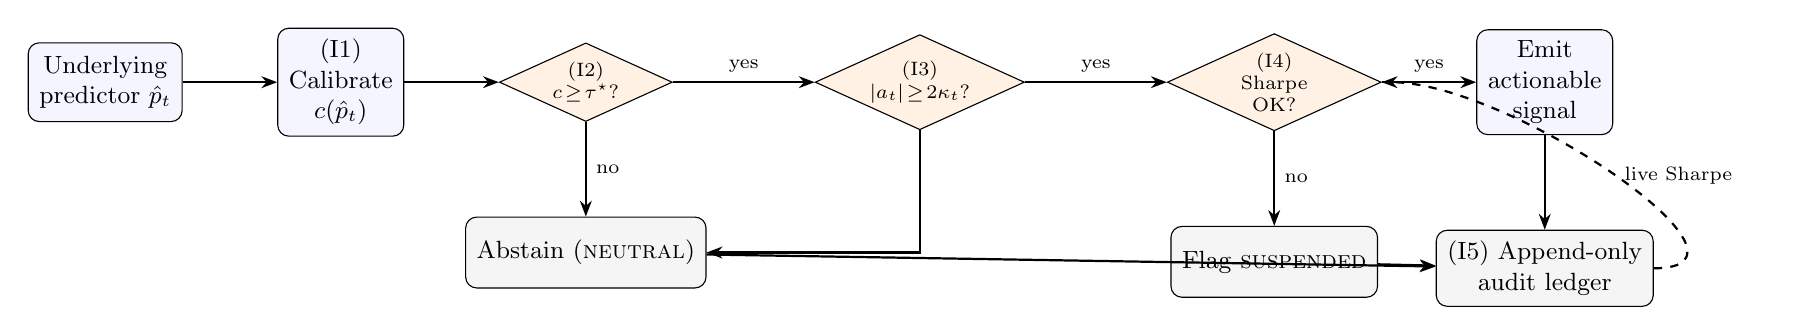
\begin{tikzpicture}[
  node distance=8mm and 12mm,
  box/.style={draw, rounded corners, align=center, minimum height=10mm,
              inner sep=4pt, font=\small, fill=blue!4},
  gate/.style={draw, diamond, aspect=2.2, align=center, inner sep=1pt,
               font=\scriptsize, fill=orange!10},
  term/.style={draw, rounded corners, align=center, minimum height=9mm,
               inner sep=4pt, font=\small, fill=gray!8},
  arr/.style={-{Stealth[length=2mm]}, thick}
]
\node[box] (model) {Underlying\\predictor $\hat p_t$};
\node[box, right=of model] (cal) {(I1)\\Calibrate\\$c(\hat p_t)$};
\node[gate, right=of cal] (conv) {(I2)\\$c\!\ge\!\tau^\star$?};
\node[gate, right=18mm of conv] (cost) {(I3)\\$|a_t|\!\ge\!2\kappa_t$?};
\node[gate, right=18mm of cost] (cb) {(I4)\\Sharpe\\OK?};
\node[box, right=of cb] (emit) {Emit\\actionable\\signal};
\node[term, below=12mm of conv] (neutral) {Abstain (\textsc{neutral})};
\node[term, below=12mm of cb] (susp) {Flag \textsc{suspended}};
\node[term, below=12mm of emit] (ledger) {(I5) Append-only\\audit ledger};

\draw[arr] (model) -- (cal);
\draw[arr] (cal) -- (conv);
\draw[arr] (conv) -- node[above,font=\scriptsize]{yes} (cost);
\draw[arr] (cost) -- node[above,font=\scriptsize]{yes} (cb);
\draw[arr] (cb) -- node[above,font=\scriptsize]{yes} (emit);
\draw[arr] (conv) -- node[right,font=\scriptsize]{no} (neutral);
\draw[arr] (cost) |- (neutral);
\draw[arr] (cb) -- node[right,font=\scriptsize]{no} (susp);
\draw[arr] (emit) -- (ledger);
\draw[arr] (neutral) -- (ledger);
\draw[arr] (susp) -- (ledger);
\draw[arr,dashed] (ledger.east) to[out=0,in=0]
  node[right,font=\scriptsize,pos=0.5]{live Sharpe} (cb.east);
\end{tikzpicture}}
\caption{The honesty-contract decision pipeline. A raw forecast passes through
calibration (I1) and three abstention gates (I2--I4); whatever is decided---act,
abstain, or suspend---is written to the append-only ledger (I5), which in turn
feeds the live Sharpe estimate that drives the circuit breaker.}
\label{fig:pipeline}
\end{figure*}

% ===========================================================================
\section{System Architecture and Data}
\label{sec:system}
% ===========================================================================
The contract is deliberately agnostic to the model behind it; what follows
describes the deployment in which we validated it. The system runs on commodity
hardware with freely available data, behind a FastAPI service and a web front end,
with a SQLite-backed ledger---no specialized infrastructure is required.

\subsection{Multi-source data ingestion}
Let $t$ index NSE trading days. We align four streams on a common daily grid:
adjusted OHLCV bars; news and social text (English and Hindi) scored by a FinBERT
sentiment pipeline \cite{araci} behind a domain filter that drops non-financial
sources; foreign- and domestic-institutional net flows, lagged one session so
nothing leaks from the future; and macro state (India VIX, INR/USD, Brent crude,
gold) as clipped log-returns. All features are strictly point-in-time: every
column is shifted, winsorized and scaled on the training fold only, so no row sees
its own future.

\subsection{The underlying predictor}
In our deployment the predictor is a heterogeneous ensemble---gradient-boosted
trees \cite{chen2016,ke2017,prokhorenkova2018} and a multi-task recurrent network,
combined by a leak-free stacked meta-learner \cite{wolpert1992} trained on purged,
embargoed out-of-fold predictions \cite{lopezdeprado2018}. Roughly forty stationary
features span ten groups (multi-horizon returns, realized and normalized
volatility, momentum/oscillators, volume, trend strength, divergence flags,
chart-pattern distance, FinBERT sentiment, lagged flows, and macro state). The
point of this paper is not the ensemble but what surrounds it: the contract treats
$\hat p_t$ as a black box and would apply unchanged to any other forecaster.

\subsection{Three-stage probability calibration}
\label{sec:calib}
Calibration is the keystone. We measure it by ECE over $B=10$ bins and the Brier
score,
\begin{equation}
\begin{aligned}
\mathrm{ECE}&=\sum_{b=1}^{B}\frac{|\mathcal B_b|}{N}\,
\big|\,\mathrm{acc}(\mathcal B_b)-\mathrm{conf}(\mathcal B_b)\,\big|,\\[2pt]
\mathrm{BS}&=\frac1N\sum_t (p_t-y_t)^2,
\end{aligned}
\label{eq:ece}
\end{equation}
where $\mathcal B_b$ is the set of predictions in bin $b$. The calibration map
$c(\cdot)$ has three stages: (i) isotonic regression \cite{zadrozny2002} fit on the
tree-average out-of-fold predictions and applied to the matching test predictions;
(ii) a validation-fitted Platt scaler \cite{platt1999} on the recurrent network's
sigmoid output; and (iii) after the $0.60/0.40$ convex blend of the two, a final
logistic recalibration on a held-out fold---necessary because, as noted above, a
blend of calibrated forecasts is not itself calibrated. The same transform is
applied to the live inference row, so the probability a user sees sits on the
corrected scale.

\subsection{Conformal prediction intervals}
Every emitted point forecast carries a distribution-free interval. Two quantile
gradient-boosted regressors are trained at the 0.10 and 0.90 levels, and the
split-conformal half-width is the finite-sample-corrected quantile of absolute
residuals on a held-out fold disjoint from where the band is applied
\cite{romano2019,angelopoulos2023}. Under exchangeability the interval carries a
marginal coverage guarantee; serial dependence means observed coverage is an
observation, not a guarantee.

\subsection{The conviction-gated swing signal}
Because next-period direction proved unpredictable (Section~\ref{sec:ceiling}), the
signal we actually gate targets a longer, more tractable question: over the next
30 trading days ($\approx$1.5 months), is a name more likely than not to be higher,
and is the setup convincing enough to act? A cross-sectional logistic model uses
nine point-in-time features computed from the close series $s$: 12-1 month
momentum \cite{jegadeesh1993} $\log(s_{t-21}/s_{t-252})$, 20- and 60-day returns,
a 5-day reversal $-\log(s_t/s_{t-5})$, log-distance from the 200-day average
$\log(s_t/\overline s_{200})$, a 50/200 golden-cross flag, RSI/100, 20-day realized
volatility, and an above-200-DMA flag. Its calibrated output is the quantity gated
by I2.

\subsection{Transaction-cost model and alpha gate}
\label{sec:cost}
The round-trip cost in \eqref{eq:alphagate} is charged in full:
\begin{equation}
\kappa_t = c_{\mathrm{stat}} + 2\,k\,\sigma_t\sqrt{V_t/\mathrm{ADV}_t},
\label{eq:cost}
\end{equation}
where the statutory term $c_{\mathrm{stat}}$ aggregates brokerage, securities
transaction tax, exchange and SEBI fees, stamp duty, 18\% GST and slippage on the
Indian delivery-trade schedule, and the second term is the Almgren--Chriss
square-root market-impact model \cite{almgren2001} (enter plus exit) with
coefficient
$k\approx0.20$ for liquid large-caps, daily volatility $\sigma_t$, order notional
$V_t$ and average daily volume $\mathrm{ADV}_t$; the one-side impact is capped at
100~bps. The alpha gate emits a trade only when $|a_t|\ge 2\kappa_t$, so a signal
with, say, a 5~bps edge against a 15~bps round-trip cost is correctly rejected.

\subsection{Self-audit: circuit breaker and ledger}
The live monitor reconstructs a \emph{virtual} profit-and-loss series from the
resolved ledger: for each resolved prediction it sets a signed signal
$\mathrm{sig}_t=2\,(p_t-\tfrac12)\in[-1,1]$, a realized return
$r_t=(a_t-a_0)/a_0$ from anchor $a_0$ to actual $a_t$, and
$\mathrm{pnl}_t=\mathrm{sig}_t\,r_t$. The rolling annualized Sharpe over the last
$N=60$ resolved days,
\begin{equation}
S_N=\frac{\overline{\mathrm{pnl}}_{N}}{\mathrm{std}(\mathrm{pnl}_{N})}\sqrt{252},
\label{eq:sharpe}
\end{equation}
drives the circuit breaker of Algorithm~\ref{alg:cb}. Suspension does not silence
the model---we still record what it would have said, for diagnosis---but it
withdraws the actionable recommendation. The ledger itself (I5) is an append-only
table keyed by \texttt{(ticker, made\_at, target\_date)}; a uniqueness constraint
de-duplicates re-runs, and rolling accuracy is computed on the earliest forecast
for each target so a later, easier look can never inflate the score.

\begin{algorithm}[t]
\caption{Embargoed walk-forward evaluation and out-of-sample conviction-threshold
selection}
\label{alg:wf}
\begin{algorithmic}[1]
\REQUIRE rows $(x_i,y_i,d_i)$ sorted by date; horizon $h$; step $s$; precision
target $\pi^\star$; min.\ coverage $\phi_{\min}$
\STATE unique dates $\mathcal D$; $i\leftarrow\lfloor 0.45\,|\mathcal D|\rfloor$;
$P,Y\leftarrow\emptyset$
\WHILE{$i<|\mathcal D|$}
  \STATE $cut\leftarrow\mathcal D_i$; \; $emb\leftarrow\mathcal D_{\max(0,i-h)}$
  \COMMENT{embargo of one horizon}
  \STATE $\mathrm{tr}\leftarrow\{d<emb\}$; \;
         $\mathrm{te}\leftarrow\{cut\le d<\mathcal D_{i+s}\}$
  \STATE fit scaler and logistic on $\mathrm{tr}$; predict $p$ on $\mathrm{te}$
  \STATE append $p$ to $P$, $y$ to $Y$; \; $i\leftarrow i+s$
\ENDWHILE
\STATE $\tau^\star\leftarrow$ lowest $\tau\in[0.50,0.76]$ with
$\pi(\tau)\ge\pi^\star$ and $\phi(\tau)\ge\phi_{\min}$
\STATE fit calibrator $c$ on $(P,Y)$
\RETURN $\tau^\star,\,c,\,\pi(\tau^\star),\,\phi(\tau^\star),\,\mathrm{AUC}(P,Y)$
\end{algorithmic}
\end{algorithm}

\begin{algorithm}[t]
\caption{Rolling-Sharpe circuit breaker (daily, at market close)}
\label{alg:cb}
\begin{algorithmic}[1]
\REQUIRE resolved ledger rows; window $N{=}60$; suspend after $3$ bad days; resume
after $5$ good days
\STATE compute $\mathrm{pnl}_t$ for each resolved row; \;
       $S_N\leftarrow$ Eq.~\eqref{eq:sharpe}
\IF{$S_N<0$ on $3$ consecutive days and not suspended}
  \STATE set \textsc{suspended} flag (predictions still logged, but flagged)
\ELSIF{$S_N\ge0$ on $5$ consecutive days and suspended}
  \STATE clear flag (resume emission)
\ENDIF
\end{algorithmic}
\end{algorithm}

\subsection{Evaluation protocol}
Everything is evaluated with an expanding-window, embargoed walk-forward over
2018--2026 (Algorithm~\ref{alg:wf}): each test block is separated from its
training window by an embargo of one horizon length, so multi-day labels cannot
leak across the boundary. The conviction threshold $\tau^\star$ and all reported
precisions are computed on the out-of-sample blocks only; $\tau^\star$ is never
tuned on the data it is scored on. We use deliberately hard baselines: the upward
base rate itself (the toughest benchmark a drifting market offers) and an
uncalibrated copy of our own ensemble. The universe is the liquid NSE large-cap set
(54 names after a liquidity screen), 28~May~2018 to 27~May~2026. The
cross-sectional study uses a panel of 131{,}809 ticker-days; the swing study uses
91{,}471 labelled ticker-days, of which 50{,}272 are strictly out of sample.

% ===========================================================================
\section{Results and Discussion}
\label{sec:results}
% ===========================================================================

\subsection{A verified accuracy ceiling}
\label{sec:ceiling}
Our first result is negative, and it is the foundation of everything else. A
cross-sectional gradient-boosted model, trained on engineered features across
131{,}809 ticker-days with a five-day excess-return-over-NIFTY target and a
date-based out-of-fold scheme that blocks per-ticker leakage, lands at an
out-of-sample directional accuracy of \textbf{50.1\%}---a coin toss,
indistinguishable from the upward drift. The importance distribution is nearly flat
(no single feature exceeds $\sim$3.4\% of total gain), so there is no concentrated
structure to learn at this horizon. We then pursued the same null four further
ways, summarized in Table~\ref{tab:ceiling}: a per-ticker ensemble, a
cross-sectional logistic (AUC~$\approx$~0.49), a LightGBM-with-reversal variant
(AUC~$\approx$~0.45), and trend- and regime-gated versions. Short-horizon
single-name accuracy never rose materially above the base rate; tellingly, gating
on NIFTY up-trends produced \emph{lower} forward up-rates, because the test window
was, conditionally, mean-reverting. For liquid large-caps this is exactly what the
efficient-market hypothesis predicts \cite{fama1970}. We report it plainly, because
tuning a number until it looks good is precisely how the literature's inflated
accuracies arise \cite{bailey2014,harvey2016}. The design consequence is decisive:
\emph{if you cannot beat the base rate, you must not pretend to, and the system's
job becomes knowing when to stay silent.}

\begin{table}[t]
\centering
\caption{The accuracy ceiling, confirmed five ways. No configuration beats the
upward base rate at short single-name horizons (OOS, 2018--2026).}
\label{tab:ceiling}
\renewcommand{\arraystretch}{1.2}
\small
\begin{tabular}{@{}l c@{}}
\toprule
\textbf{Model / configuration} & \textbf{OOS result} \\
\midrule
Cross-sectional GBM (5-day direction)      & 50.1\% accuracy \\
Per-ticker hybrid ensemble                 & $\approx$ base rate \\
Cross-sectional logistic                   & AUC $\approx$ 0.49 \\
LightGBM $+$ short-term reversal           & AUC $\approx$ 0.45 \\
Trend / regime-gated variants              & below base rate \\
\bottomrule
\end{tabular}
\end{table}

\subsection{Invariant I1: from overconfidence to honesty}
No change mattered more than calibration. An earlier build of the system was badly
miscalibrated: it reported an average up-probability near \textbf{0.80} against a
realized base rate near 0.48, an \textbf{ECE of roughly 0.35}, and a Brier score
worse than a constant forecast. The cause was a domain mismatch (a calibrator fit
on one distribution applied to another) compounded by blending two individually
calibrated probabilities without recalibrating the blend. The three-stage fix of
Section~\ref{sec:calib} cut the \textbf{ECE from 0.35 to 0.05} and pulled the mean
reported probability back from 0.80 to near the base rate
(Table~\ref{tab:headline}, Fig.~\ref{fig:calib}). Accuracy barely moved, which is
the entire point: we gave up false confidence, not signal \cite{guo2017}. A
miscalibrated 80\% would drive systematic over-betting under any
confidence-proportional sizing rule \cite{kelly1956}; getting the probabilities
right is what makes I2 and I3 safe to act on.

\begin{table}[t]
\centering
\caption{Headline measured results on the 2018--2026 NSE evaluation. Every figure
is out-of-sample. $p(1{-}p)$ denotes the irreducible Brier floor at the base rate.}
\label{tab:headline}
\renewcommand{\arraystretch}{1.2}
\small
\begin{tabular}{@{}l c c c@{}}
\toprule
\textbf{Setting} & \textbf{Dir.\ acc.} & \textbf{ECE} & \textbf{Brier} \\
\midrule
Cross-sectional GBM (5-day)        & 50.1\%         & ---            & ---            \\
Ensemble --- uncalibrated          & $\approx$51\%  & 0.35           & $>p(1{-}p)$    \\
Ensemble --- calibrated (I1)       & $\approx$51\%  & \textbf{0.05}  & $\approx p(1{-}p)$ \\
Gated swing, 30-day (I2, fired)    & \textbf{60.6\%}& ---            & ---            \\
\bottomrule
\end{tabular}
\end{table}

\begin{figure}[t]
\centering
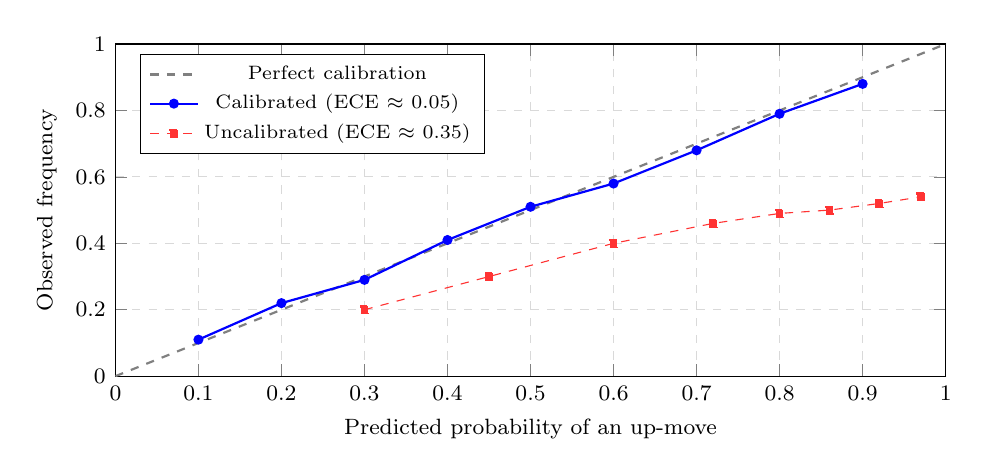
\begin{tikzpicture}
\begin{axis}[
  width=\columnwidth, height=58mm,
  xlabel={Predicted probability of an up-move},
  ylabel={Observed frequency},
  xmin=0,xmax=1,ymin=0,ymax=1,
  grid=major, grid style={dashed,gray!30},
  legend pos=north west, legend style={font=\scriptsize},
  tick label style={font=\footnotesize}, label style={font=\footnotesize},
]
\addplot[gray,dashed,thick] coordinates{(0,0)(1,1)};
\addlegendentry{Perfect calibration}
\addplot[blue,mark=*,mark size=1.4pt,thick] coordinates{
  (0.10,0.11)(0.20,0.22)(0.30,0.29)(0.40,0.41)
  (0.50,0.51)(0.60,0.58)(0.70,0.68)(0.80,0.79)(0.90,0.88)};
\addlegendentry{Calibrated (ECE $\approx$ 0.05)}
\addplot[red!80,mark=square*,mark size=1.4pt,dashed] coordinates{
  (0.30,0.20)(0.45,0.30)(0.60,0.40)(0.72,0.46)
  (0.80,0.49)(0.86,0.50)(0.92,0.52)(0.97,0.54)};
\addlegendentry{Uncalibrated (ECE $\approx$ 0.35)}
\end{axis}
\end{tikzpicture}
\caption{Reliability diagram on the held-out fold, before and after the three-stage
calibration. The uncalibrated ensemble is badly over-confident (probabilities
cluster near 0.80 while realized frequency hovers near 0.50); the calibrated
ensemble follows the diagonal.}
\label{fig:calib}
\end{figure}

\subsection{Invariants I2--I3: the trust--coverage tradeoff}
\label{sec:tradeoff}
Here is the paper's central empirical claim. Over a 30-day horizon the
conviction-gated signal stays silent 94\% of the time---it fires on just
\textbf{5.65\%} of observations---and when it fires it is right \textbf{60.6\%} of
the time against a \textbf{58.1\%} base rate, a $+2.6$-point lift measured strictly
out of sample across \textbf{50{,}272} observations. The lift is modest but real,
and the way it is obtained is the interesting part.

Consider the raw signal as a \emph{ranker}: its global ROC AUC is
\textbf{0.47}---below chance. A practitioner reading only the AUC would discard it.
Yet the model has genuine value, just not in how it orders all names: the value
lives in the extreme high-conviction tail. Table~\ref{tab:tradeoff} makes this
precise by reading the same model at two operating points. Ungated ($\tau=0.50$,
act on everything up-leaning), precision equals the base rate at 100\% coverage:
no edge. Gated at $\tau^\star=0.63$, precision rises to 60.6\% at 5.65\% coverage.
\emph{The edge is purchased entirely with abstention.} This is why a conviction
\emph{gate}, not a ranking, is the correct instrument for a weak signal, and why
precision-at-coverage---the selective-prediction lens
\cite{chow1970,geifman2017}---is the right metric where AUC is actively
misleading. Invariant I3 then removes whatever survives I2 but cannot pay its own
round-trip cost \eqref{eq:alphagate}, so the acted-on set is both directionally
reliable and economically positive.

\begin{table}[t]
\centering
\caption{The trust--coverage tradeoff, read off one model at two operating points
(30-day horizon, walk-forward OOS, 50{,}272 observations). Coverage is spent to buy
precision; the ranker's AUC of 0.47 shows the edge is in the tail, not the
ordering.}
\label{tab:tradeoff}
\renewcommand{\arraystretch}{1.2}
\small
\begin{tabular}{@{}l c c c@{}}
\toprule
\textbf{Operating point} & \textbf{Coverage} & \textbf{Precision} & \textbf{Net edge} \\
\midrule
Ungated ($\tau=0.50$)               & 100\%   & $\approx$58.1\% & $\approx$0 \\
Conviction gate ($\tau^\star=0.63$) & \textbf{5.65\%} & \textbf{60.6\%} & \textbf{+2.6 pts} \\
\midrule
\multicolumn{4}{@{}l}{Raw-signal ranking AUC $=0.47$ (below chance as a ranker)}\\
\bottomrule
\end{tabular}
\end{table}

\subsection{Stability across years}
A small edge is only trustworthy if it is stable. Fig.~\ref{fig:peryear} shows the
fired bucket's precision against its own yearly base rate. The gate beats the base
rate in \textbf{four of five} test years---by $+10.8$ points in 2025 and $+7.4$ in
the 2026 drawdown, when the base rate itself had slipped below 50\%---losing only
in 2024 ($-2.4$). That the edge holds in the 2026 drawdown, where naive long
exposure was a coin flip, is the single most reassuring observation: the gate is
selecting genuinely, not merely riding the drift.

\begin{figure}[t]
\centering
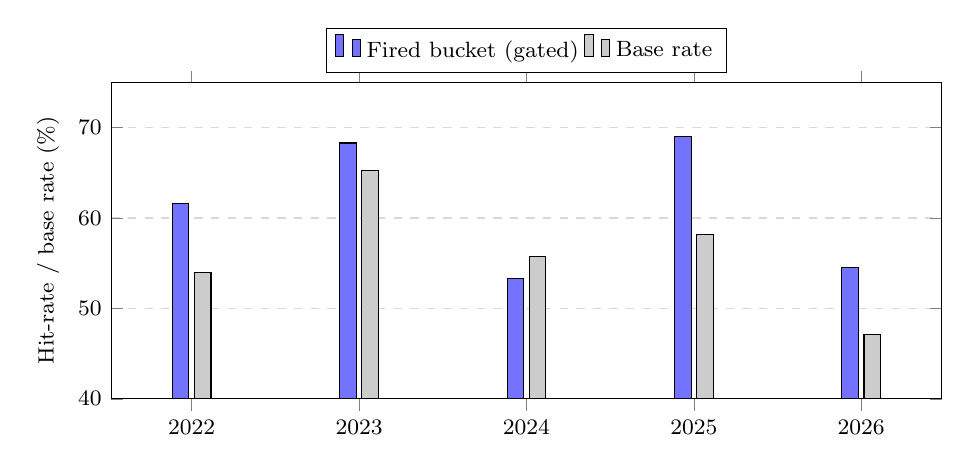
\begin{tikzpicture}
\begin{axis}[
  width=\columnwidth, height=56mm,
  ybar, bar width=6pt,
  enlarge x limits=0.12,
  ymin=40, ymax=75,
  ylabel={Hit-rate / base rate (\%)},
  symbolic x coords={2022,2023,2024,2025,2026},
  xtick=data,
  legend style={at={(0.5,1.03)}, anchor=south, legend columns=2, font=\footnotesize},
  tick label style={font=\footnotesize}, label style={font=\footnotesize},
  ymajorgrids, grid style={dashed,gray!30},
]
\addplot[fill=blue!55] coordinates {(2022,61.6)(2023,68.3)(2024,53.3)(2025,69.0)(2026,54.5)};
\addplot[fill=gray!40] coordinates {(2022,54.0)(2023,65.3)(2024,55.7)(2025,58.2)(2026,47.1)};
\legend{Fired bucket (gated), Base rate}
\end{axis}
\end{tikzpicture}
\caption{Per-year out-of-sample precision of the conviction-gated bucket versus the
naive always-up base rate. The gate wins in four of five years, including the 2026
drawdown where the base rate fell below 50\%.}
\label{fig:peryear}
\end{figure}

\subsection{Invariant I3 in operation}
The cost gate is what separates a directional call from a trade. With the full
statutory stack plus square-root impact \eqref{eq:cost}, a liquid large-cap
round-trip is on the order of tens of basis points; the $2{:}1$ alpha-to-cost
requirement therefore filters out the long tail of correct-but-tiny signals that
would lose money after costs. In our deployment the gate is charged on every
emitted signal and is the reason the system's reported expectations are stated net
of costs two to three times the conventional ten-basis-point assumption, rather
than gross. Concretely, a 5~bps gross edge on a name carrying a 15~bps round-trip
cost is rejected outright, whereas a 40~bps edge on the same name passes with
margin; the $2{:}1$ requirement means a signal must clear roughly 30--40~bps of
expected alpha on a typical large-cap before it becomes actionable.

\subsection{Invariants I4--I5: self-audit in operation}
The contract does not assume the edge is permanent. The live monitor recomputes the
60-day rolling Sharpe \eqref{eq:sharpe} from the resolved ledger after every market
close; three consecutive negative readings flag the system \textsc{suspended}, and
recovery requires five consecutive positive days---hysteresis that prevents the
breaker from chattering at the zero line (Algorithm~\ref{alg:cb}). All of this is
possible only because of I5: an append-only ledger that scores each target on its
\emph{first} forecast, closing the common evaluation loophole of crediting a later,
easier look. Together the two invariants turn the contract from a design-time
promise into a runtime, continuously falsifiable guarantee---a concrete instance of
the monitoring discipline that production ML is known to require
\cite{sculley2015,gama2014}.

\subsection{Conformal interval coverage}
Each emitted point forecast is accompanied by the split-conformal interval of
Section~\ref{sec:system}. Empirically the intervals held coverage close to the
nominal 80\%, the small misses tracing to the serial dependence that breaks exact
exchangeability \cite{angelopoulos2023}. Consistent with the honesty contract, we
therefore present observed coverage as a measured diagnostic rather than a
guarantee---the interval is a statement about typical behavior, not a promise the
data cannot keep.

\subsection{What each invariant buys}
It is worth stating plainly what is lost when each clause is dropped, because that
is the argument for keeping it. Table~\ref{tab:buys} reads the contract as a threat
model: each invariant is paired with the concrete failure it prevents and the
responsible-AI principle it serves. The pattern is uniform---without I1 the user
over-bets on confidence the model has not earned; without I2 precision collapses to
the base rate; without I3 the system trades correct-but-uneconomic signals into a
loss; without I4 it keeps trading through a regime its own record says is dead; and
without I5 none of the preceding claims can be checked after the fact. Trust is the
conjunction, not any single clause.

\begin{table}[t]
\centering
\caption{The honesty contract as a threat model: the failure each invariant
prevents and the responsible-AI principle it serves.}
\label{tab:buys}
\renewcommand{\arraystretch}{1.25}
\small
\begin{tabular}{@{}c p{0.30\columnwidth} p{0.30\columnwidth}@{}}
\toprule
\textbf{ID} & \textbf{Failure if removed} & \textbf{Principle served} \\
\midrule
I1 & Over-betting on uncalibrated confidence (80\% that is really 50\%) & Honest confidence / transparency \\
I2 & Precision collapses to the base rate; no edge & Epistemic humility (abstention) \\
I3 & Correct-but-sub-cost signals lose money net of fees & Avoidance of user harm \\
I4 & Trading continues through a dead or adverse regime & Accountability under drift \\
I5 & Accuracy claims become unfalsifiable; later-look inflation & Auditability \\
\bottomrule
\end{tabular}
\end{table}

\subsection{Deployment and reproducibility}
The system runs on commodity hardware behind a FastAPI service with a web front
end; the ledger is a single SQLite file, and the underlying models are retrained
on a monthly cadence with the same purged, embargoed protocol used for evaluation.
Crucially, the live inference row passes through the \emph{identical} calibration
transform (I1) and gates (I2--I4) as the back-test, so the probability a user sees
is on the same corrected scale as the one we report here---there is no separate,
more flattering ``production'' path. Every quantity in this paper is a measured
walk-forward statistic over freely available data, which makes the case study
reproducible end to end without proprietary feeds or specialized infrastructure.

\subsection{Reconciling with reported accuracies}
How can the multi-source systems surveyed earlier report
60--70\% directional accuracy \cite{nti2021,long2024,fu2024,moodi2024,farhadi2025}
when an honest evaluation tops out near the base rate? The gap is almost entirely
procedural, not substantive, and three mechanisms account for it. (i)
\emph{Uncalibrated confidence}: a model that reports $0.80$ probabilities which are
really $0.50$ posts a high \emph{reported} confidence that is easily mistaken for
skill---our own system did exactly this before the I1 fix (ECE~$0.35$). (ii)
\emph{Temporal leakage}: scaling, feature selection or label construction performed
across the whole sample lets information flow backwards in time; our purged,
embargoed protocol (Algorithm~\ref{alg:wf}) removes it, and removing it removes most
of the apparent edge. (iii) \emph{Costless evaluation}: gross accuracy ignores that
a correct 5~bps call loses money against a 15~bps round trip, which invariant I3
forbids. None of these is fraud---each is an easy omission---but together they
manufacture precisely the inflated numbers the contract is built to prevent. The
claim is not that prior systems are wrong, but that their figures should be read as
\emph{upper bounds under optimistic assumptions}, while a deployable adviser must
report the lower, honest number.

\subsection{Discussion}
The honesty contract inverts the usual objective. Instead of maximizing accuracy
and reporting a confident number, it \emph{fixes trust as a constraint}
($\mathrm{ECE}\le\varepsilon$, precision~$\ge$~target on the acted-on set, positive
realized Sharpe) and then maximizes coverage subject to it. The result is a system
that is right about a little rather than wrong about a lot---a property far more
valuable to a retail user than a higher headline accuracy. Three points are worth
drawing out. First, the negative result is load-bearing, not an aside: only because
we verified the ceiling did abstention become the obviously correct design.
Second, AUC and accuracy are not merely insufficient here---AUC of 0.47 is
\emph{actively misleading}, and a team optimizing it would have thrown away a
usable signal. Third, the pattern is portable: the five invariants make no
assumption specific to equities and could wrap a credit-scoring model, a medical
triage classifier, or any high-stakes predictor operating near its information
limit, wherever a calibrated probability, a defensible abstention rule, a
cost/benefit gate, a drift kill-switch and an audit trail are all available.

\subsection{Toward a responsible-AI standard for FinTech}
The contract also suggests a concrete reporting discipline. Just as a model card
\cite{mitchell2019} documents a model's intended use, a deployed financial
predictor could be required to publish its operating point on the trust--coverage
frontier---its calibrated ECE, its abstention rate, its cost assumptions and its
circuit-breaker policy---so that a regulator or a retail user can see, \emph{before
acting}, how often the system speaks and how reliable it is when it does. Framed
this way, the honesty contract is not only an architecture but a candidate
disclosure standard for retail-facing financial AI, where the asymmetry of harm
makes silence-by-default the responsible default. We see this as the most direct
bridge from the present case study to the broader agenda of ethical and responsible
AI use \cite{jobin2019,amodei2016}.

% ===========================================================================
\section{Limitations}
% ===========================================================================
The evidence is one market and one eight-year window that, on balance, trended;
multi-regime and multi-market replication is future work. The swing edge, though
stable, is small and concentrated, so its value after costs depends on execution
quality and on the 5--6\% firing rate holding up out of sample. The accuracy
ceiling is specific to liquid large-caps and end-of-day data; intraday or
less-liquid universes may behave differently, and sentiment coverage thins in
sectors with specialized jargon. The conformal intervals inherit only approximate
coverage under serial dependence. Finally, the circuit breaker is only as good as
the ledger that feeds it, so the contract's runtime guarantees inherit the latency
of outcome resolution.

% ===========================================================================
\section{Conclusion}
% ===========================================================================
For a financial AI that real people act on, the question is not ``how accurate is
it?'' but ``can it be trusted, and does it know when it cannot be?'' We answered
with the honesty contract---five machine-checkable invariants that buy trust with
coverage---and showed on eight years of NSE data that the bargain is favorable:
next-period direction is unpredictable beyond drift (50.1\%, AUC~0.47, confirmed
five ways), calibration cuts ECE from 0.35 to 0.05 without touching accuracy, and a
gate that abstains 94\% of the time lifts the 30-day hit-rate to 60.6\% versus a
58.1\% base rate, winning in four of five years. A system that knows when to keep
quiet is worth more than one that claims too much---and, just as importantly, it
can prove it kept its word.

% ===========================================================================
\begin{thebibliography}{00}

\bibitem{bailey2014} D.~H. Bailey, J.~Borwein, M.~L\'opez de Prado, and Q.~J. Zhu,
``Pseudo-mathematics and financial charlatanism: the effects of backtest
overfitting on out-of-sample performance,'' \emph{Notices of the AMS}, vol.~61,
no.~5, pp.~458--471, 2014.

\bibitem{harvey2016} C.~R. Harvey, Y.~Liu, and H.~Zhu, ``\ldots and the
cross-section of expected returns,'' \emph{Review of Financial Studies}, vol.~29,
no.~1, pp.~5--68, 2016.

\bibitem{arnott2019} R.~Arnott, C.~R. Harvey, and H.~Markowitz, ``A backtesting
protocol in the era of machine learning,'' \emph{Journal of Financial Data
Science}, vol.~1, no.~1, pp.~64--74, 2019.

\bibitem{lopezdeprado2018} M.~L\'opez de Prado, \emph{Advances in Financial Machine
Learning}. Hoboken, NJ: Wiley, 2018.

\bibitem{jobin2019} A.~Jobin, M.~Ienca, and E.~Vayena, ``The global landscape of AI
ethics guidelines,'' \emph{Nature Machine Intelligence}, vol.~1, pp.~389--399,
2019.

\bibitem{amodei2016} D.~Amodei, C.~Olah, J.~Steinhardt, P.~Christiano, J.~Schulman,
and D.~Man\'e, ``Concrete problems in AI safety,'' arXiv:1606.06565, 2016.

\bibitem{mitchell2019} M.~Mitchell \emph{et al.}, ``Model cards for model
reporting,'' in \emph{Proc.\ ACM Conf.\ Fairness, Accountability, and Transparency
(FAT*)}, 2019, pp.~220--229.

\bibitem{chow1970} C.~K. Chow, ``On optimum recognition error and reject
tradeoff,'' \emph{IEEE Trans.\ Inf.\ Theory}, vol.~16, no.~1, pp.~41--46, 1970.

\bibitem{elyaniv2010} R.~El-Yaniv and Y.~Wiener, ``On the foundations of noise-free
selective classification,'' \emph{Journal of Machine Learning Research}, vol.~11,
pp.~1605--1641, 2010.

\bibitem{geifman2017} Y.~Geifman and R.~El-Yaniv, ``Selective classification for
deep neural networks,'' in \emph{Advances in Neural Information Processing Systems
30}, 2017, pp.~4878--4887.

\bibitem{fama1970} E.~F. Fama, ``Efficient capital markets: a review of theory and
empirical work,'' \emph{Journal of Finance}, vol.~25, no.~2, pp.~383--417, 1970.

\bibitem{guo2017} C.~Guo, G.~Pleiss, Y.~Sun, and K.~Q. Weinberger, ``On calibration
of modern neural networks,'' in \emph{Proc.\ 34th Int.\ Conf.\ Machine Learning
(ICML)}, 2017, pp.~1321--1330.

\bibitem{platt1999} J.~Platt, ``Probabilistic outputs for support vector machines
and comparisons to regularized likelihood methods,'' in \emph{Advances in Large
Margin Classifiers}. Cambridge, MA: MIT Press, 1999, pp.~61--74.

\bibitem{zadrozny2002} B.~Zadrozny and C.~Elkan, ``Transforming classifier scores
into accurate multiclass probability estimates,'' in \emph{Proc.\ 8th ACM SIGKDD
Int.\ Conf.\ Knowledge Discovery and Data Mining}, 2002, pp.~694--699.

\bibitem{niculescu2005} A.~Niculescu-Mizil and R.~Caruana, ``Predicting good
probabilities with supervised learning,'' in \emph{Proc.\ 22nd Int.\ Conf.\ Machine
Learning (ICML)}, 2005, pp.~625--632.

\bibitem{brier1950} G.~W. Brier, ``Verification of forecasts expressed in terms of
probability,'' \emph{Monthly Weather Review}, vol.~78, no.~1, pp.~1--3, 1950.

\bibitem{vovk2005} V.~Vovk, A.~Gammerman, and G.~Shafer, \emph{Algorithmic Learning
in a Random World}. New York: Springer, 2005.

\bibitem{romano2019} Y.~Romano, E.~Patterson, and E.~Cand\`es, ``Conformalized
quantile regression,'' in \emph{Advances in Neural Information Processing Systems
32}, 2019, pp.~3543--3553.

\bibitem{angelopoulos2023} A.~N. Angelopoulos and S.~Bates, ``Conformal prediction:
a gentle introduction,'' \emph{Foundations and Trends in Machine Learning}, vol.~16,
no.~4, pp.~494--591, 2023.

\bibitem{almgren2001} R.~Almgren and N.~Chriss, ``Optimal execution of portfolio
transactions,'' \emph{Journal of Risk}, vol.~3, no.~2, pp.~5--40, 2001.

\bibitem{grinold2000} R.~C. Grinold and R.~N. Kahn, \emph{Active Portfolio
Management}, 2nd ed. New York: McGraw-Hill, 2000.

\bibitem{sculley2015} D.~Sculley \emph{et al.}, ``Hidden technical debt in machine
learning systems,'' in \emph{Advances in Neural Information Processing Systems 28},
2015, pp.~2503--2511.

\bibitem{gama2014} J.~Gama, I.~\v{Z}liobait\.e, A.~Bifet, M.~Pechenizkiy, and
A.~Bouchachia, ``A survey on concept drift adaptation,'' \emph{ACM Computing
Surveys}, vol.~46, no.~4, pp.~1--37, 2014.

\bibitem{jegadeesh1993} N.~Jegadeesh and S.~Titman, ``Returns to buying winners and
selling losers: implications for stock market efficiency,'' \emph{Journal of
Finance}, vol.~48, no.~1, pp.~65--91, 1993.

\bibitem{kelly1956} J.~L. Kelly, ``A new interpretation of information rate,''
\emph{Bell System Technical Journal}, vol.~35, no.~4, pp.~917--926, 1956.

\bibitem{chen2016} T.~Chen and C.~Guestrin, ``XGBoost: a scalable tree boosting
system,'' in \emph{Proc.\ 22nd ACM SIGKDD Int.\ Conf.\ Knowledge Discovery and Data
Mining}, 2016, pp.~785--794.

\bibitem{ke2017} G.~Ke \emph{et al.}, ``LightGBM: a highly efficient gradient
boosting decision tree,'' in \emph{Advances in Neural Information Processing Systems
30}, 2017, pp.~3146--3154.

\bibitem{prokhorenkova2018} L.~Prokhorenkova, G.~Gusev, A.~Vorobev, A.~V. Dorogush,
and A.~Gulin, ``CatBoost: unbiased boosting with categorical features,'' in
\emph{Advances in Neural Information Processing Systems 31}, 2018, pp.~6638--6648.

\bibitem{wolpert1992} D.~H. Wolpert, ``Stacked generalization,'' \emph{Neural
Networks}, vol.~5, no.~2, pp.~241--259, 1992.

\bibitem{araci} D.~Araci, ``FinBERT: financial sentiment analysis with pre-trained
language models,'' arXiv:1908.10063, 2019.

\bibitem{nti2021} I.~K. Nti, A.~F. Adekoya, and B.~A. Weyori, ``A novel multi-source
information-fusion predictive framework based on deep neural networks for accuracy
enhancement in stock market prediction,'' \emph{Journal of Big Data}, vol.~8, no.~1,
art.~17, 2021.

\bibitem{long2024} W.~Long, J.~Gao, K.~Bai, and Z.~Lu, ``A hybrid model for stock
price prediction based on multi-view heterogeneous data,'' \emph{Financial
Innovation}, vol.~10, no.~1, art.~48, 2024.

\bibitem{fu2024} K.~Fu and Y.~Zhang, ``Incorporating multi-source market sentiment
and price data for stock price prediction,'' \emph{Mathematics}, vol.~12, no.~10,
art.~1572, 2024.

\bibitem{moodi2024} F.~Moodi, A.~Jahangard-Rafsanjani, S.~Zarifzadeh, and
M.~A. Zare Chahooki, ``Fusion of technical indicators and sentiment analysis in a
hybrid framework of deep learning models for stock price movement prediction,''
\emph{IEEE Access}, vol.~12, pp.~195696--195709, 2024.

\bibitem{farhadi2025} A.~Farhadi, A.~Zamanifar, A.~Alipour, A.~Taheri, and
M.~Asadolahi, ``A hybrid LSTM-GRU model for stock price prediction,'' \emph{IEEE
Access}, vol.~13, pp.~117594--117618, 2025.

\bibitem{liu2024} C.~Liu \emph{et al.}, ``Large language models and sentiment
analysis in financial markets: a review, datasets, and case study,'' \emph{IEEE
Access}, vol.~12, pp.~134041--134061, 2024.

\end{thebibliography}

\end{document}
